In $13\,\mathrm{TeV}$ proton-proton collisions the $t$-channel mode ~\cite{firstharris,firsttramontano,firstkidonakis} is the most abundant of the three single top quark production mechanisms predicted in the standard model of elementary particle physics (SM). And it is the one with the most striking final state topology because of the presence, 
within acceptance, of a light quark recoiling against the top quark. Figure~\ref{fig:FG} shows two Feynman diagrams of $t$-channel single top quark production. Depending on whether the calculation includes b (sea-) quarks inside the proton or not the process starts directly with a light quark and a b quark (five flavour scheme, Fig.~\ref{fig:FG}(a)) or with a light quark and a gluon, which splits into a pair of b quark and antiquark (four flavor scheme, Fig.~\ref{fig:FG}(b)).

The study of single top quark production provides a unique possibility to investigate many aspects 
of top-quark physics that cannot be easily studied in $\ttbar$ production. All three channels 
are directly related to the modulus squared of the CKM matrix element $V_{tb}$, allowing for a 
direct measurement of this quantity and thus for a further test of the SM, 
and in particular of the assumption that only three quark families exist~\cite{Alwall:2006bx,Holdom:2009rf}. 
One can investigate the tWb vertex structure and flavour-changing neutral current (FCNC) couplings in the production processes.
A review of many opportunities to observe new physics 
from deviations in the expected cross sections of the $t$- and $s$-channel modes can be found, e.g., in Ref.~\cite{Tait:2000sh}. 

	\begin{figure}[h]
	  \begin{center}
	    \subfigure[]{
	     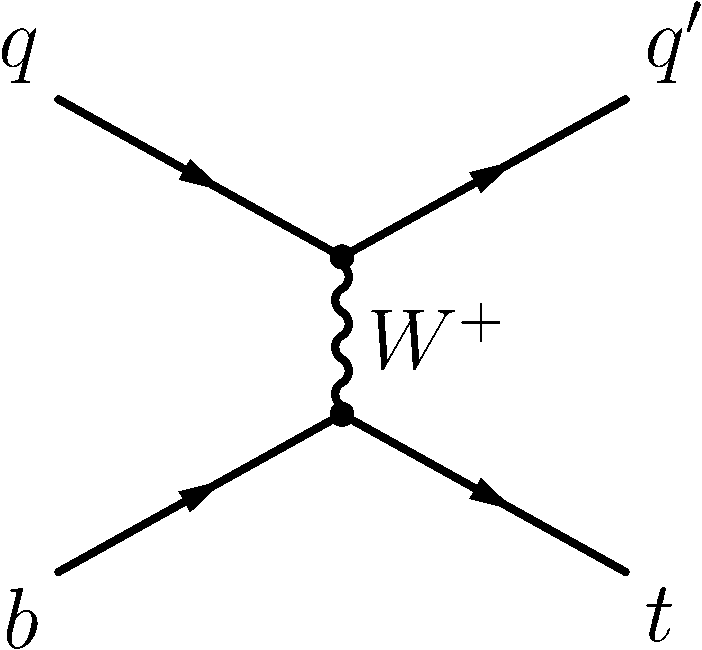
\includegraphics[width=0.18\textwidth]{figures/tchannel22}
		\hspace{0.5cm}}
		\subfigure[]{
	    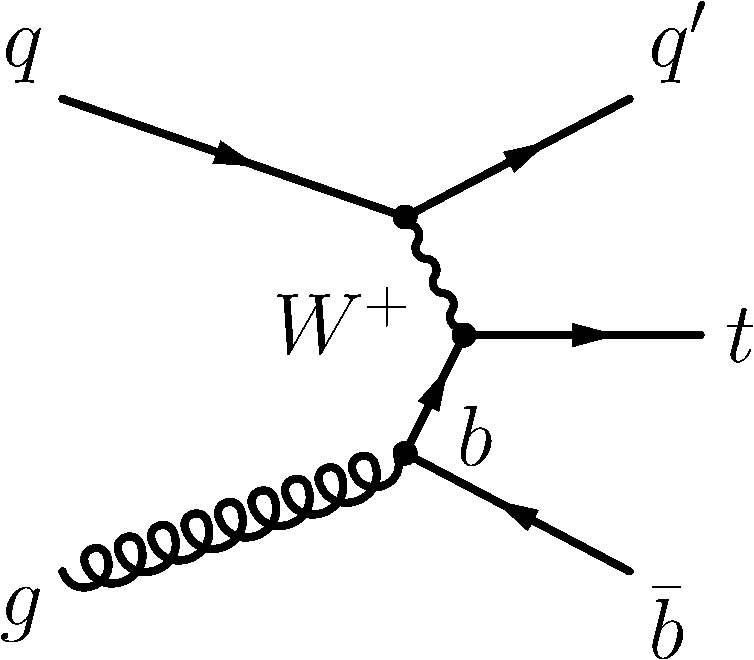
\includegraphics[width=0.18\textwidth]{figures/tchannel23}}
	    \hfill
	    \caption{\label{fig:FG}Leading order Feynman diagrams for single top quark production via the $t$-channel in the five flavour scheme (a) and in the four flavour scheme (b). The latter can also be seen as an NLO contribution in the four flavor scheme.}
	  \end{center}
	\end{figure}

The aim of the analysis described in this note is to measure the inclusive single-top quark $t$-channel production cross section.

In this note the $t$-channel is considered as signal process, while the $s$-channel and W-associated production are included among the background processes. 
The analysis strategy is similar to the one applied in Refs.~\cite{TOP-11-021,TOP-12-038}, where the precision measurements of $t$-channel single-top-quark cross section has been performed at 7 and 8 TeV respectively.

This measurement is based on the leptonic decay channel in which the W boson produced in the top-quark decay further decays producing a muon and one or more neutrinos (via $\tau$ lepton decay chains) in the final state.
%The branching ratio of the top quark with a muon in or electron the final state is $B(\mathrm{t}\to\mu\nu \mathrm{b})=0.1080$~\cite{pdg} for each.
The cascade decay $\mathrm{t}\to\tau\to\mu$ is considered as part of the signal.

The signal fraction is extracted using a maximum likelihood fit of the distribution of the absolute value 
of the pseudorapidity of the light jet stemming from the parton recoiling against the top quark, $\etalj$, 
which allows to discriminate between single top $t$-channel and its main background contributions.
The expected distributions of $\etalj$ are determined from either simulation or from data.

Control samples are defined in order to check the distributions of the variables used in the analysis for the main background sources, 
and an ad-hoc study is performed on the effect of pile up interactions on the analysis.

The note is organized as follows:
\begin{itemize}
\item Sec.~\ref{sec:samples} describes the data and samples of simulated events and the software framework used;
\item Sec.~\ref{sec:selection} describes the event selection and the method used for the reconstruction of the top quark, defining the main variables
used in the analysis;
%\item Sec.~\ref{sec:2J0T} describes the control region used to check our W$+$jets distributions and our QCD extraction procedure.
%\item Sec.~\ref{sec:3JNT} describes the control region used to check our top-antitop distributions.
\item Sec.~\ref{sec:muonEff} describes the determination of the muon trigger
  and ID efficiencies.
\item Sec.~\ref{sec:controlplots} describes the control regions to check the \wjets and \ttbar~backgrounds.
\item Sec.~\ref{sec:qcd} describes the data-driven modelling of the $\qcd$ background and the estimation of its contribution to the signal region.
\item Sec.~\ref{sec:WHFExtraction} describes the modelling of the $\wjets$ background;
\item Sec.~\ref{sec:xsection} presents the cross section extraction based on a template fit to \etalj;
\item Sec.~\ref{sec:syst} explains in details how the systematic uncertainties have been estimated; 
\item Sec.~\ref{sec:results} summarizes the results.
\end{itemize}


%{\bf Disclaimer:}
%Many of the numbers and plots in this document are based on studies on pseudodata. They will updated using real collision data as soon as sufficient statistics are available. All MC-based plots with pseudo data are normalized to the aimed at luminosity of $1\,\mathrm{fb}^{-1}$. Plots with real data include all currently available data, corresponding to an integrated luminosity of around $20\,\mathrm{pb}^{-1}$.

%\include{todolist}
